% ==================================
%           Chapter 1B.3
%  Circulation in the Blood Vessels
%       Created by Michael Tang
%            2025.01.12
% ==================================

\subsubsection{1B.3 Circulation in the Blood Vessels}
\paragraph{Types of Blood Vessels}
\begin{itemize}
    \item[1.] \textbf{\underline{Arteries} (动脉)}
    \begin{itemize}
        \item \textbf{Function:} Carry blood away from the heart (usually \underline{oxygenated} (充满氧气的), except for
        \underline{pulmonary} (肺部) and \underline{umbilical} (脐带) arteries).
        \item \textbf{Structure:}
        \begin{itemize}
            \item Thick walls with \underline{elastic fibres} (弹性纤维), \underline{smooth muscle} (平滑肌), and
            \underline{collagen} (胶原蛋白) to \underline{withstand} (承受) high pressure.
            \item Narrow \underline{lumen} (管腔) to maintain high pressure.
        \end{itemize}
        \begin{figure}[H]
            \centering
            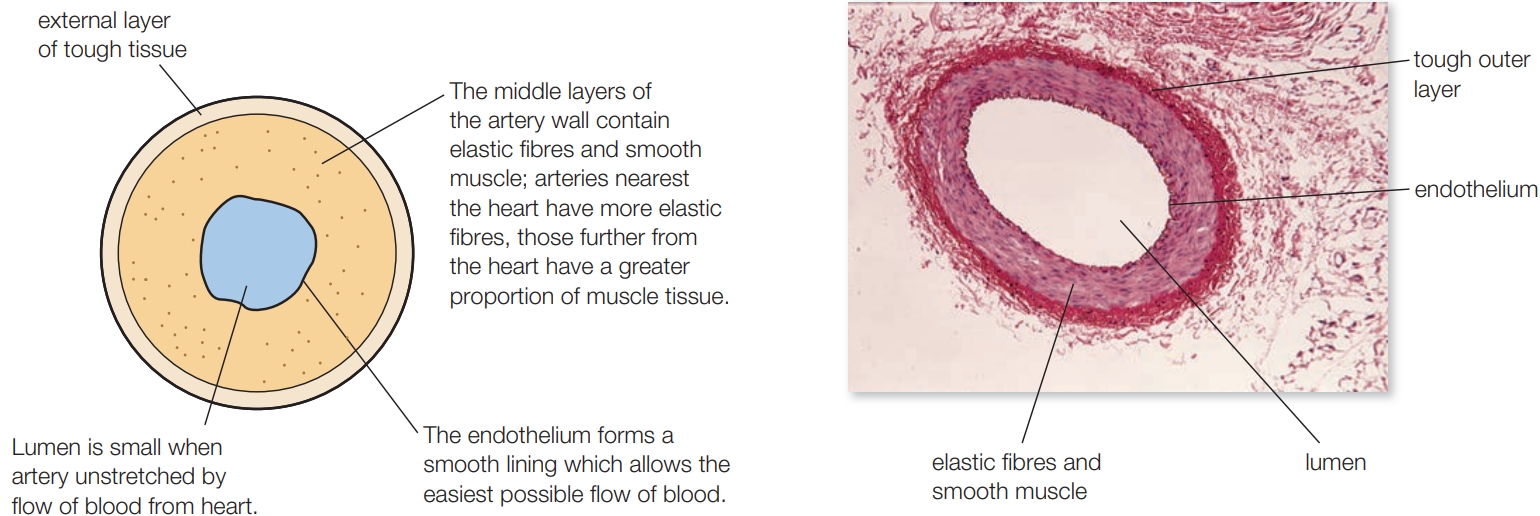
\includegraphics[scale=0.2]{Biology/1B/Images/1B-3-1.png}
            \caption{The structure of an artery means it is adapted to \underline{cope} (处理) with the \underline{surging} (涌动)
            of the blood as the heart pumps.}
        \end{figure}
        \item \textbf{Adaptations:}
        \begin{itemize}
            \item \underline{Elastic recoil} (弹性回缩) helps maintain blood flow during \underline{diastole} (舒张期).
            \item \underline{Arterioles} (小动脉) regulate blood flow to tissues by \underline{adjusting} (调整) lumen size.
        \end{itemize}
        \begin{figure}[H]
            \centering
            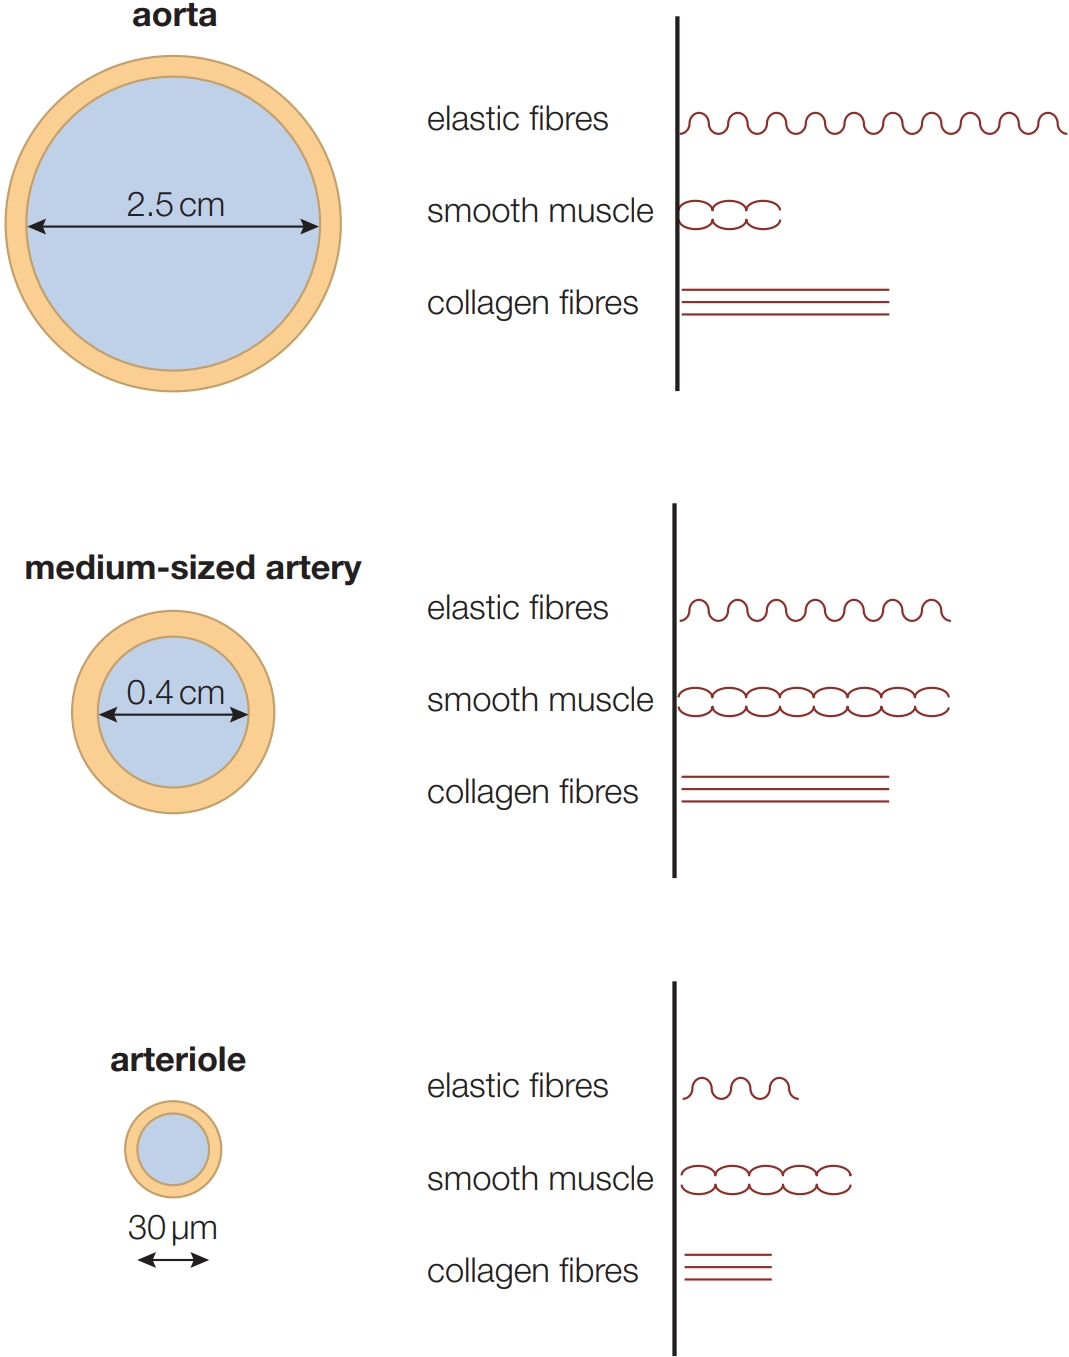
\includegraphics[scale=0.15]{Biology/1B/Images/1B-3-2.png}
            \caption{The relative proportions of different tissues in different arteries.Collagen gives general strength and
            flexibility to both arteries and veins.}
        \end{figure}
    \end{itemize}
    \item[2.] \textbf{\underline{Capillaries} (毛细血管)}
    \begin{itemize}
        \item \textbf{Function:} Facilitate exchange of substances between blood and tissues.
        \item \textbf{Structure:}
        \begin{itemize}
            \item Very thin walls (one cell thick) for efficient \underline{diffusion} (扩散).
            \item Small lumen allows red blood cells to pass through single cell, increasing contact with the
            \underline{capillary walls} (毛细血管壁).
        \end{itemize}
        \item \textbf{Adaptations:}
        \begin{itemize}
            \item Large surface area for exchange.
            \item Slow blood flow ensures more time for diffusion.
        \end{itemize}
        \begin{figure}[H]
            \centering
            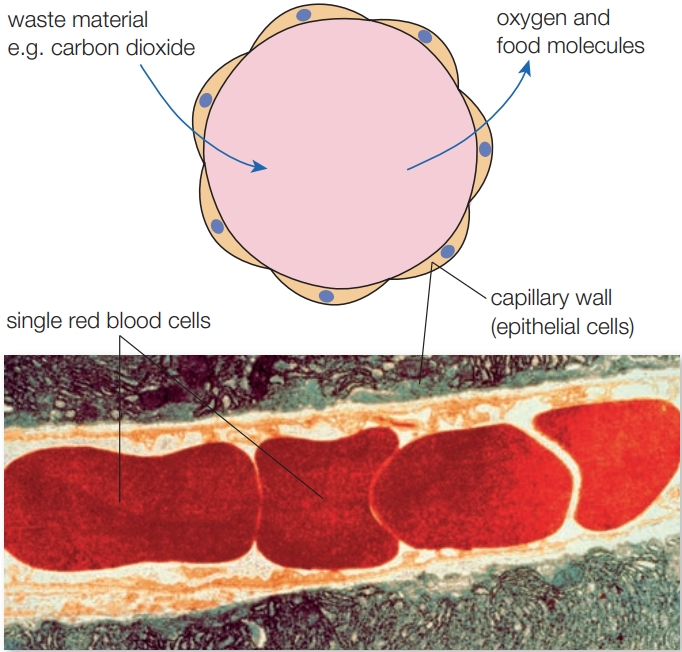
\includegraphics[scale=0.3]{Biology/1B/Images/1B-3-3.png}
            \caption{The relative proportions of different tissues in different arteries.Collagen gives general strength and
            flexibility to both arteries and veins.}
        \end{figure}
    \end{itemize}
    \item[3.] \textbf{\underline{Veins} (静脉)}
    \begin{itemize}
        \item \textbf{Function:} Carry blood back to the heart (usually \underline{deoxygenated} (缺氧的), except for pulmonary
        and umbilical veins).
        \item \textbf{Structure:}
        \begin{itemize}
            \item Thin walls with less \underline{elastic} (弹性) and muscle tissue due to lower pressure.
            \item Wide lumen to \underline{accommodate} (容纳) large volume of blood.
        \end{itemize}
        \begin{figure}[H]
            \centering
            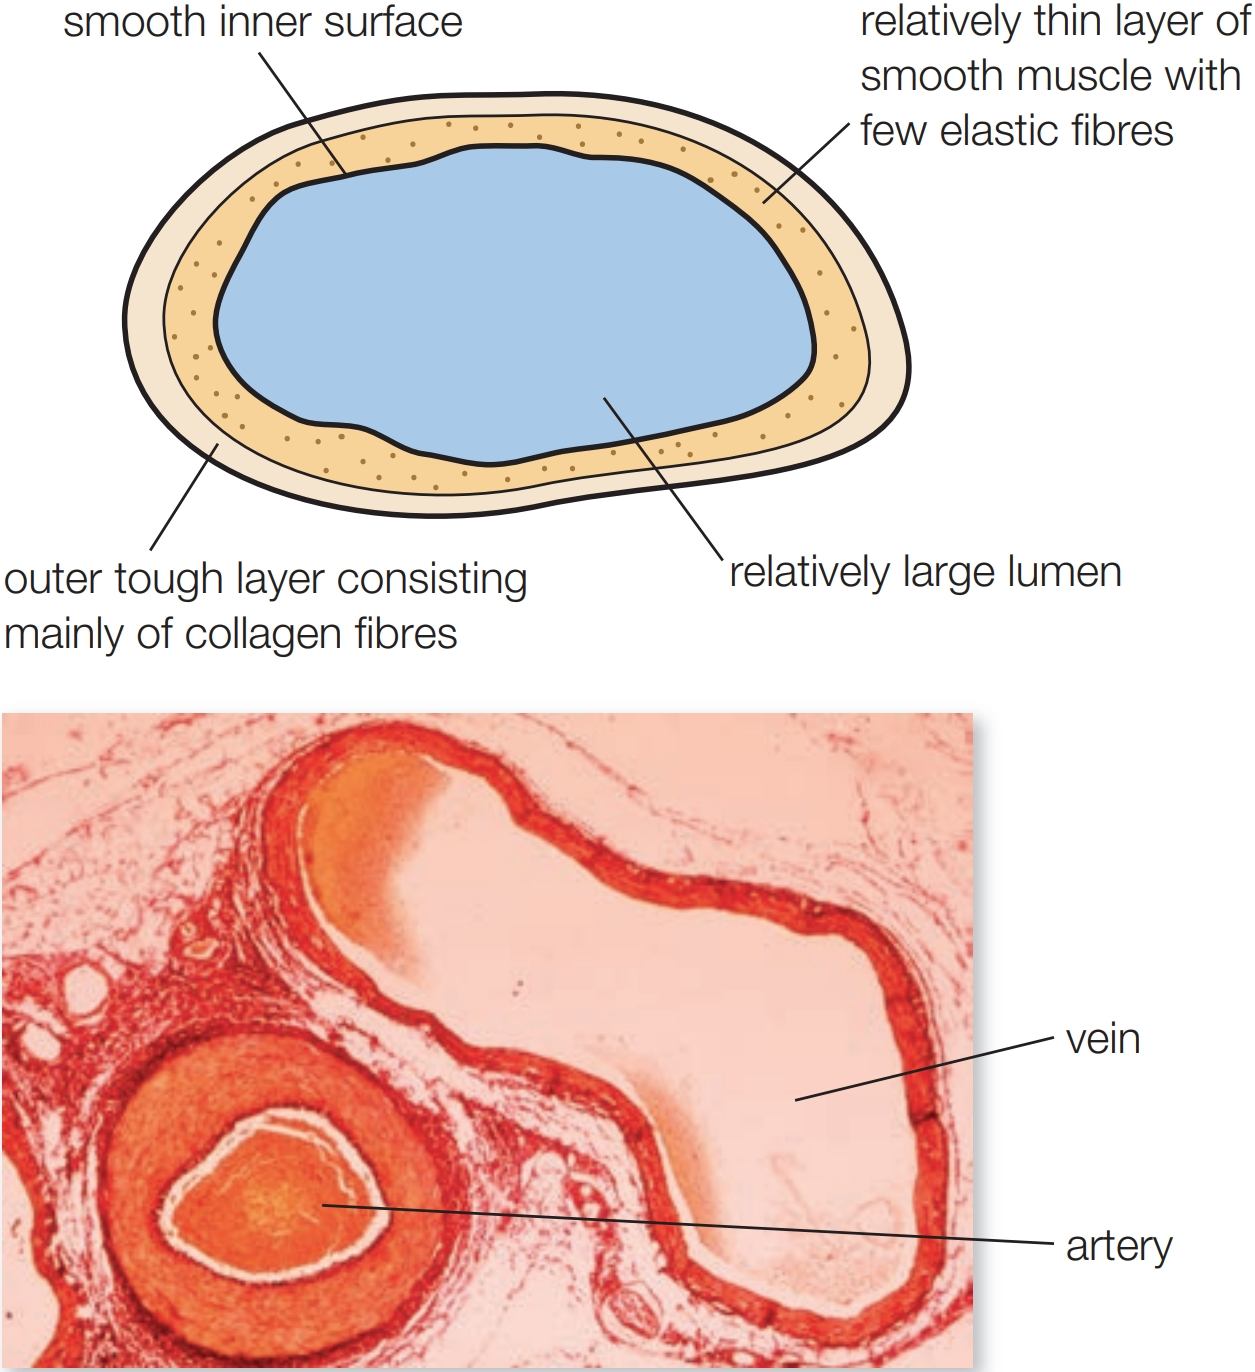
\includegraphics[scale=0.15]{Biology/1B/Images/1B-3-4.png}
            \caption{The arrangement of tissues in a vein reflects the pressure of blood in the vessel.}
        \end{figure}
    \end{itemize}
\end{itemize}

\paragraph{Key Adaptations of Blood Vessels}
\begin{itemize}
    \item \textbf{Arteries:}
    \begin{itemize}
        \item High \underline{elasticity} (弹性) for pressure \underline{surges} (涌动) from the heart.
        \item Smooth \underline{endothelium} (内皮) reduces \underline{friction} (摩擦) for efficient blood flow.
    \end{itemize}
    \begin{figure}[H]
        \centering
        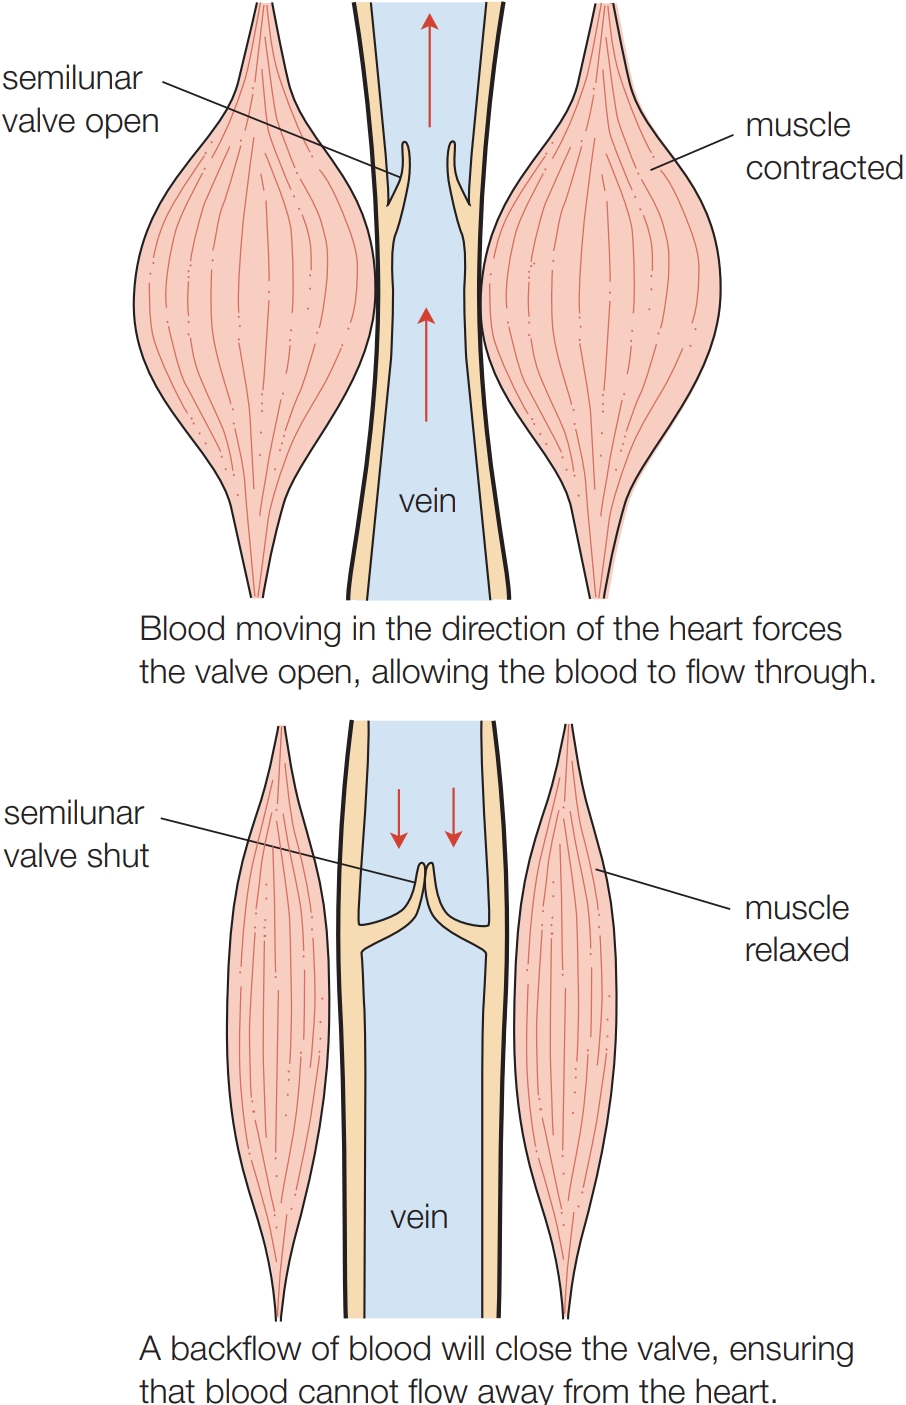
\includegraphics[scale=0.18]{Biology/1B/Images/1B-3-5.png}
        \caption{Valves in the veins make sure blood only flows in one direction - towards the heart. The contraction of large
        muscles encourages blood flow through the veins.}
    \end{figure}
    \item \textbf{Capillaries:} Short diffusion distance for gas exchange.
    \item \textbf{Veins:}
    \begin{itemize}
        \item Valves prevent backflow.
        \item Act as a \underline{reservoir} (储备) for blood (contain over 50\% of body's blood).
    \end{itemize}
\end{itemize}

\paragraph{Blood Flow Dynamics}
\begin{itemize}
    \item \textbf{Blood Pressure:} Highest in arteries, decreases in capillaries, and lowest in veins.
    \item \textbf{Velocity:} High in arteries, slows down in capillaries, and increases slightly in veins.
    \item \textbf{Surface Area:} Maximum in capillaries due to extensive branching.
\end{itemize}
\begin{figure}[H]
    \centering
    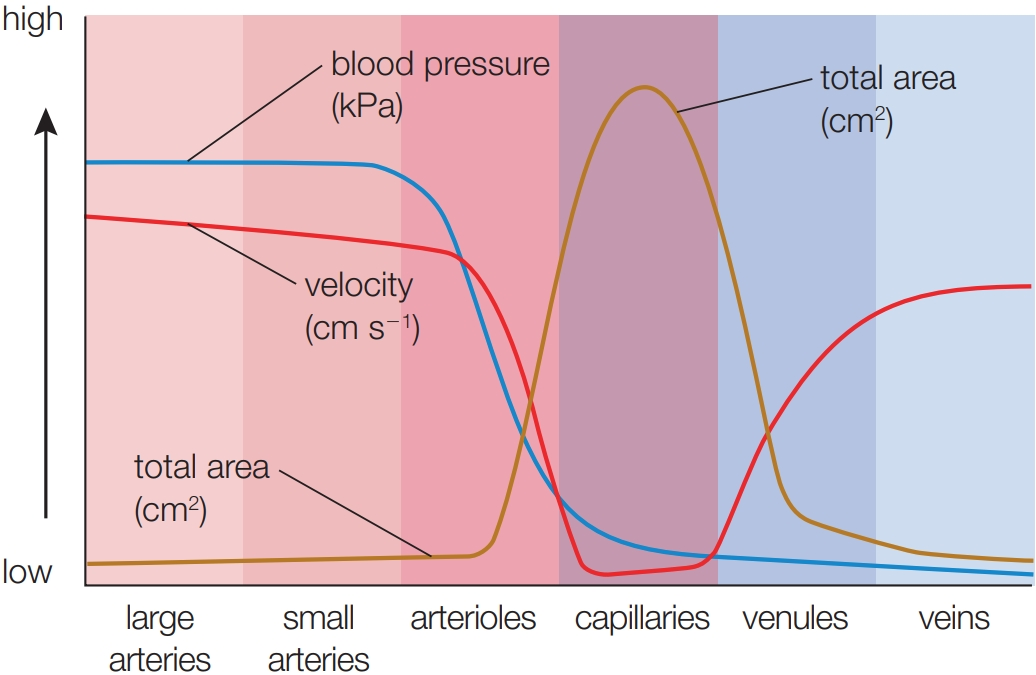
\includegraphics[scale=0.25]{Biology/1B/Images/1B-3-6.png}
    \caption{Graph to show the surface area of each major type of blood vessel in your body, along with the velocity and pressure
    of the blood travelling in them.}
\end{figure}